\documentclass[12pt, oneside]{report}
\usepackage[a4paper, width=160mm, height=245mm, top=15mm, bottom=22mm, left=30mm, right=20mm, head=3mm, foot=10mm]{geometry}
\usepackage{graphics}
\usepackage{graphicx}
\usepackage{amsmath}
\usepackage{float}
\usepackage{setspace}
\usepackage{caption}
\usepackage{subcaption}
% \usepackage[utf8]{inputenc}
% \usepackage[english]{babel}

% \usepackage{biblatex}
% \addbibresource{bibliography/bibliography.bib}

\renewcommand{\baselinestretch}{1.5}
\setlength{\parindent}{2.5cm}

\usepackage{fancyhdr}
\pagestyle{fancy}
\fancyfoot{}
\fancyfoot[CE, CO]{\thepage}
\fancyfoot[LE, LO]{Self-balancing bot}
\fancyfoot[RE, RO]{EEE F422}
\renewcommand{\headrulewidth}{0.5pt}
\renewcommand{\footrulewidth}{0.5pt}

\title{Self-balancing bot}

\author{Ravi Bharadwaj C}

\date{2018}

\pagenumbering{roman}
\setcounter{tocdepth}{4}

\begin{document}

\begin{titlepage}
	\thispagestyle{empty}
	\begin{center}
	\vspace*{1cm}

	\LARGE
	\textbf{Report Titled}

	\vspace{0.5cm}

	\Huge
	\textbf{Self balancing bot}

	\vspace{1.5cm}

	{\Large Submitted}\\
	{\Large in partial fulfillment of}\\
	{\Large the requirements of the degree of}\\
	%[0.5cm]
	{\Large Bachelor of Engineering}\\
	%{\Large (Electronics and Communication Engineering)}\\

	\vfill

\Large
	By\\
	Ravi Bharadwaj C   | 2016AAPS0244H \newline
	Akhilesh Aluvala   | 2016A3PS0281H \newline
  Akhil Raj Baranwal | 2016A8PS0372H \newline
	\vspace{1cm}
	(2018)



	%\Large
	%Dr. Alivelu M. Parimi\\
	%(Supervisor)

	\vfill

	%\Large
	%(Department of Electrical Engineering)\\
	%(2018)
\Large
\textbf{Department of Electrical Engineering, BITS Pilani-Hyderabad Campus}

	\end{center}

\end{titlepage}


\chapter*{Abstract}
This report is compiled on the basis of a hardware implemented self-balancing robot. Firstly, the report talks about the basic PID control algorithm which is used to stabilize the bot and the platform individually about thier mean positions. Further, the dynamics of a self-balancing bot are talked about in breif. Later, the mechanical construction of the bot built for this project. Further, the tuning and operation of the bot is presented at different operating conditions. Finally, the future prospects are discussed following which the report is concluded with the relevant observations and results.

\addcontentsline{toc}{chapter}{\numberline{}Abstract}

\cleardoublepage

\tableofcontents

% \listoftables
% \thispagestyle{empty}

\listoffigures
\thispagestyle{empty}

\pagenumbering{arabic}
\chapter{Introduction}
\setcounter{page}{1}
\thispagestyle{empty}

For nearly two decades research and development of self-balancing vehicles is taking place. With the upcoming availability of low-cost, high performance MEMS sensor technology, the use of inertial sensors can be used in self-balancing concepts in robotics.
A two-wheeled self-balancing system is unstable inherently.\\

After being stabilised by electronics means, they can be loaded with platforms or manipulators, working in human controlled or even completely autonomous operation, might be used in industrial autonomous transportations systems or warehouses in the future.
A two-wheeled self-balancing robot is representing a mobile inverted pendulum, which is a classic problem in dynamics and control theory.\\

Taking inspiration from present day research and utilities of a self balancing bot, the topic was chosen as a course project for the course of 'Modern Control Systems', to showcase a simple feedback controlled bot. The basic aim of the project is to build a two wheeled self-balancing bot on top of which is a mounted self-balancing platform.\\

The project showcases the use of a standard PID controller to stabilize the oscillations of the bot and hence balance it about its mean position. The same is applied to balance the self-balancing table such that it never tilts.\\


\chapter{PID control}
The PID controller (P-proportional,  I-integral, D-derivative) controller is the most widely used process control. Its control signal uses three actions on a manipulated variable to reach a specific set point.\\

\textbf{Proportional} action emits a signal proportional to the control error (control error = desired value - output value of the process).\newline
\textbf{Integral} action ensures that the steady state error is zero process, ie the process value output is equal to the desired value.\newline
The \textbf{derivative} action improves the stability of the control loop, it predicts the error value Td time forward.\\

\begin{figure}[H]
\centering
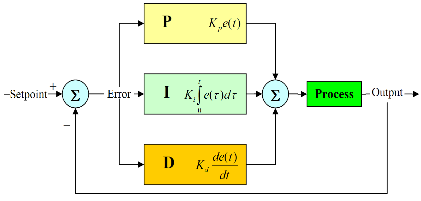
\includegraphics{images/pid}
\caption{Block diagram for a general PID controller}
\label{fig:pid}
\end{figure}

\clearpage

The PID control algorithm tries to stabilze the system about its mean position. The mean poition in the case of the self balancing bot is the pitch position at which it experiences zero torque from its own weight. The mean position in case of the self-balancing table is the position at which it is perfectly level with respect to the ground. The control algorithm is used to maintain the bot and the table individually at this mean position individually.
The response is made desirable by setting the PID values by following the steps given in the following chapter on 'Tuning'. \\

The system attempts to minimize the error by adjusting the process by relying only on the measured process variable, not on knowledge of the underlying process. Therefore, it requires minimal modelling and doesn't require excessive mathematical manipulations, making it simple to implement in low-power embedded systems.


\chapter{Bot dynamics}
\section{Modelling of self-balancing bot}

The bot consists of the two wheels connected to a body frame holding the motor drive, the power and control electronics as well as the battery. Some assumptions are made to make analysis easy.\newline

\begin{figure}[H]
\centering
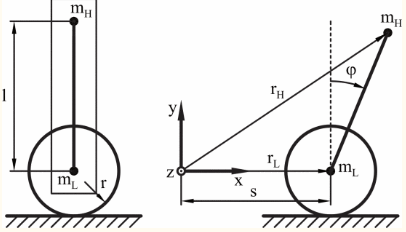
\includegraphics{images/dynamics}
\caption{Point mass model of self balancing bot}
\label{fig:dynamics}
\end{figure}

\clearpage

The assumptions are as follows (refer to figure \ref{fig:dynamics}) :
\begin{enumerate}
  \item The non-uniformly distributed mass within the body has been reduced to point masses to make analysis easy.
  \item mh and ml are connected to each other having distance l between them.
  \item The rotational inertia Jw is also taken in account.
\end{enumerate}

\section{Modelling of self-balancing platform}

The self-balancing platform is an ordinary platform with a servo attached indirectly to it through a beam. The servo is controlled by another micro-controller and this micro-controller receives feedback from a gyroscope placed on the platfrom which tells the micro-controller the displacement of the platform from its mean position. The platform here is again approximated as a point mass being displaced from its mean position.

\section{Working}

\begin{figure}[H]
\centering
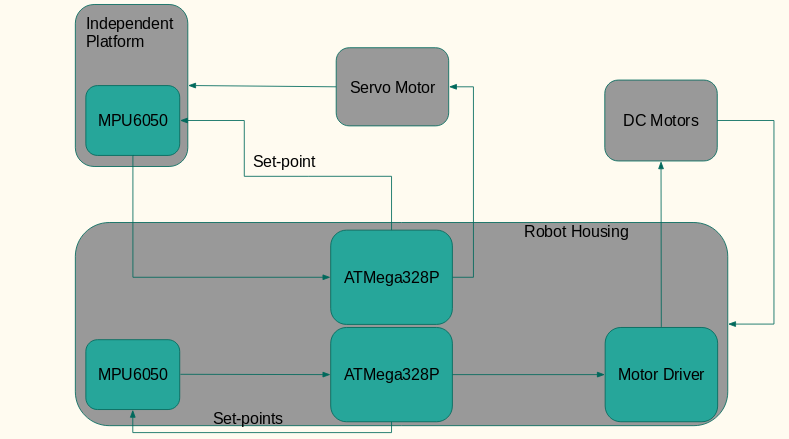
\includegraphics[width=\textwidth,height=\textheight,keepaspectratio]{images/control}
\caption{Control flow of the entire system}
\label{fig:control}
\end{figure}

Figure \ref{fig:control} shows the overall control flow of the whole system. The system works by correcting the errors in the position of the bot or platform with respect to their respective set point. \newline
If the bot is pitched forward (forward tilting motion), its new position as calculated by the gyroscope is dfferent from the set point initialized in the arduino. Hence the bot accelerates in the same direction of the tilt to compensate for the change in the the mean position. As the system is not an ideal system, the acceleration in the previous case might cause the bot to tilt in the other direction now. And hence the bot will now accelerate in a direction opposite to that before to achieve a stable state. \newline
The PID values in the control algorithm are altered on a trial and error basis to minimize these oscillations and to arrive at the stable mean position quicker.\\

The self balancing platfrom also works in a very similar manner. The main difference is that instead of giving the platfrom a linear acceleration to compensate for displacement from set point, the platfrom is simply rotated in the direction opposite to displacement using a servo. \newline
During the motion of the bot, the platfrom very rarely gets displaced from its mean position by a large enough margin to be corrected by a gyroscope. The platform is barely even displaced because :
\begin{enumerate}
  \item The structure is very rigid for there to be noticeable changes with small angular displacement.
  \item The bot accelerates with a very less acceleration value as it aims to stabilize about a point and a high acceleration would lead to the bot going out of control. This less value of acceleration is not enough to displace the platfrom from its mean position.
\end{enumerate}


\chapter{Mechanical construction}
\section{Components Used}

The components used to build the self-balancing bot and the self-balancing platform are as follows:
\begin{enumerate}
  \item Arduino UNO - 2
  \item MPU6050 Gyroscope - 2
  \item zhengk zytd520 motors - 2
  \item Orange LiPo(4100mAh, 11.1V, 35C) - 1
  \item L298N motor driver - 1
  \item MG995 servo - 1
  \item Mechanix kit - 1
  \item MM Jumper wires
  \item MF Jumper wires
\end{enumerate}

\clearpage

\section{Connections}
\subsection{Self-balancing bot}

\begin{figure}[H]
\centering
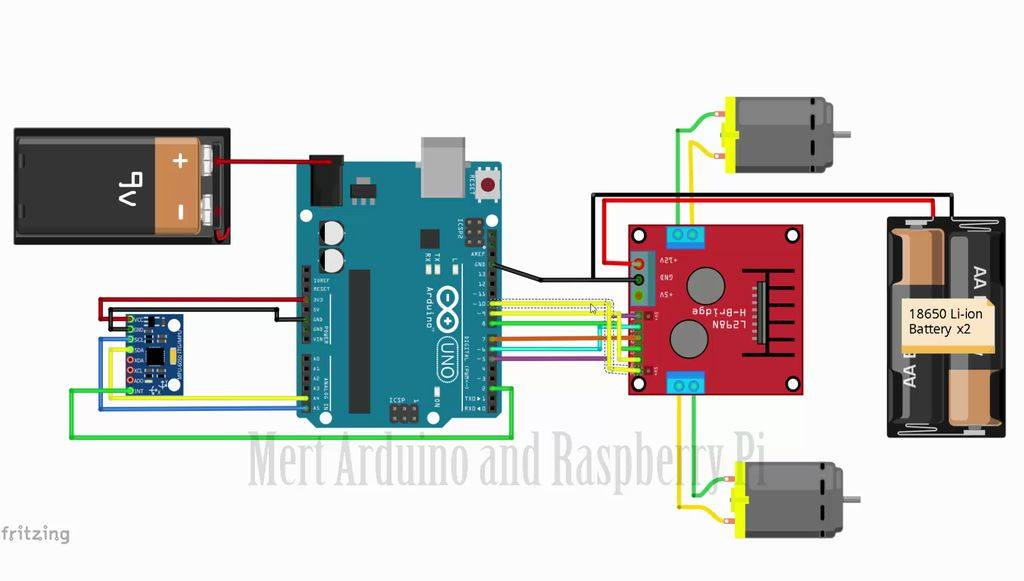
\includegraphics[width=\textwidth,height=\textheight,keepaspectratio]{images/bot-connections}
\caption{Connections for the self-balancing bot}
\label{fig:connections}
\end{figure}

The connections for the self-balancing bot are as depicted in figure \ref{fig:connections}. The Arduino UNO has been powered by connecting the 12V pin from the L298N motor driver to the \textit{Vin} pin on the arduino. The motor driver takes the 12V and GND from the battery and also has additional 5V pins.

\subsection{Self-balancing platform}

For the self-balancing platform, there is another arduino placed at the top of the bot which is connected to an MPU6050 placed on the platfrom. This helps the platform behave as an individual system. The MPU6050 on the platfrom is connected using the same connections for the MPU6050 as shown in figure \ref{fig:connections}. The servo motor is connected to pin number \textit{5} of the arduino. The arduino is powered in the same way the same way as discussed above.

\clearpage

\subsection{Final Connections}

\begin{figure}
\centering
\begin{subfigure}{.5\textwidth}
  \centering
  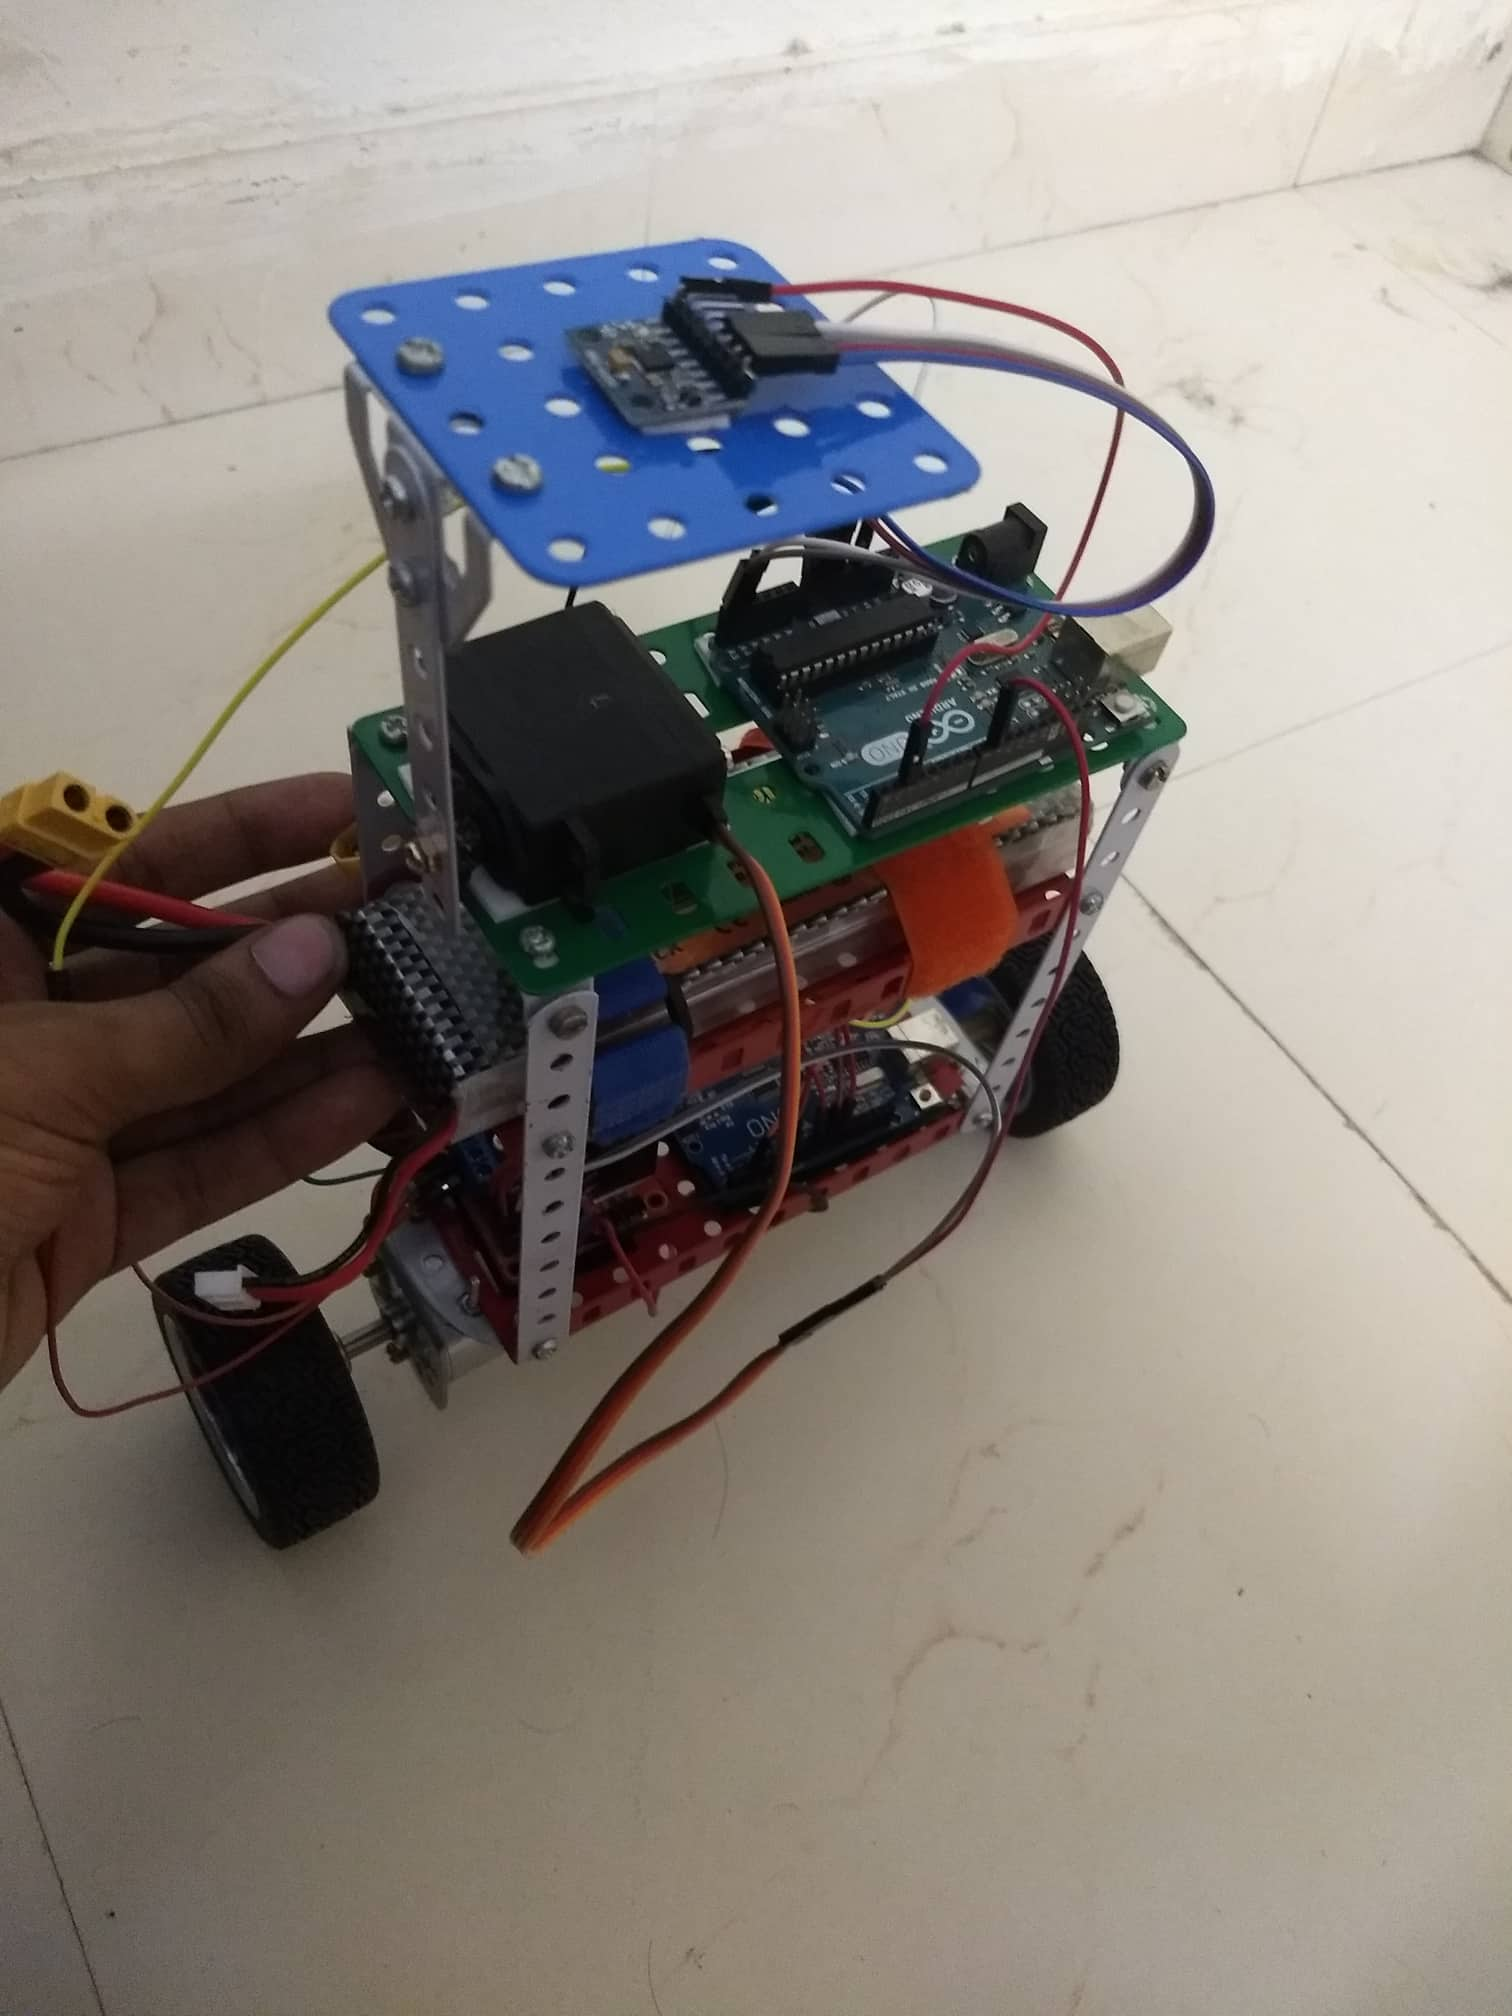
\includegraphics[width=.4\linewidth, scale = 2]{images/bot1}
  \caption{Arrangement of connections on platform}
  \label{fig:bot1}
\end{subfigure}%
\begin{subfigure}{.5\textwidth}
  \centering
  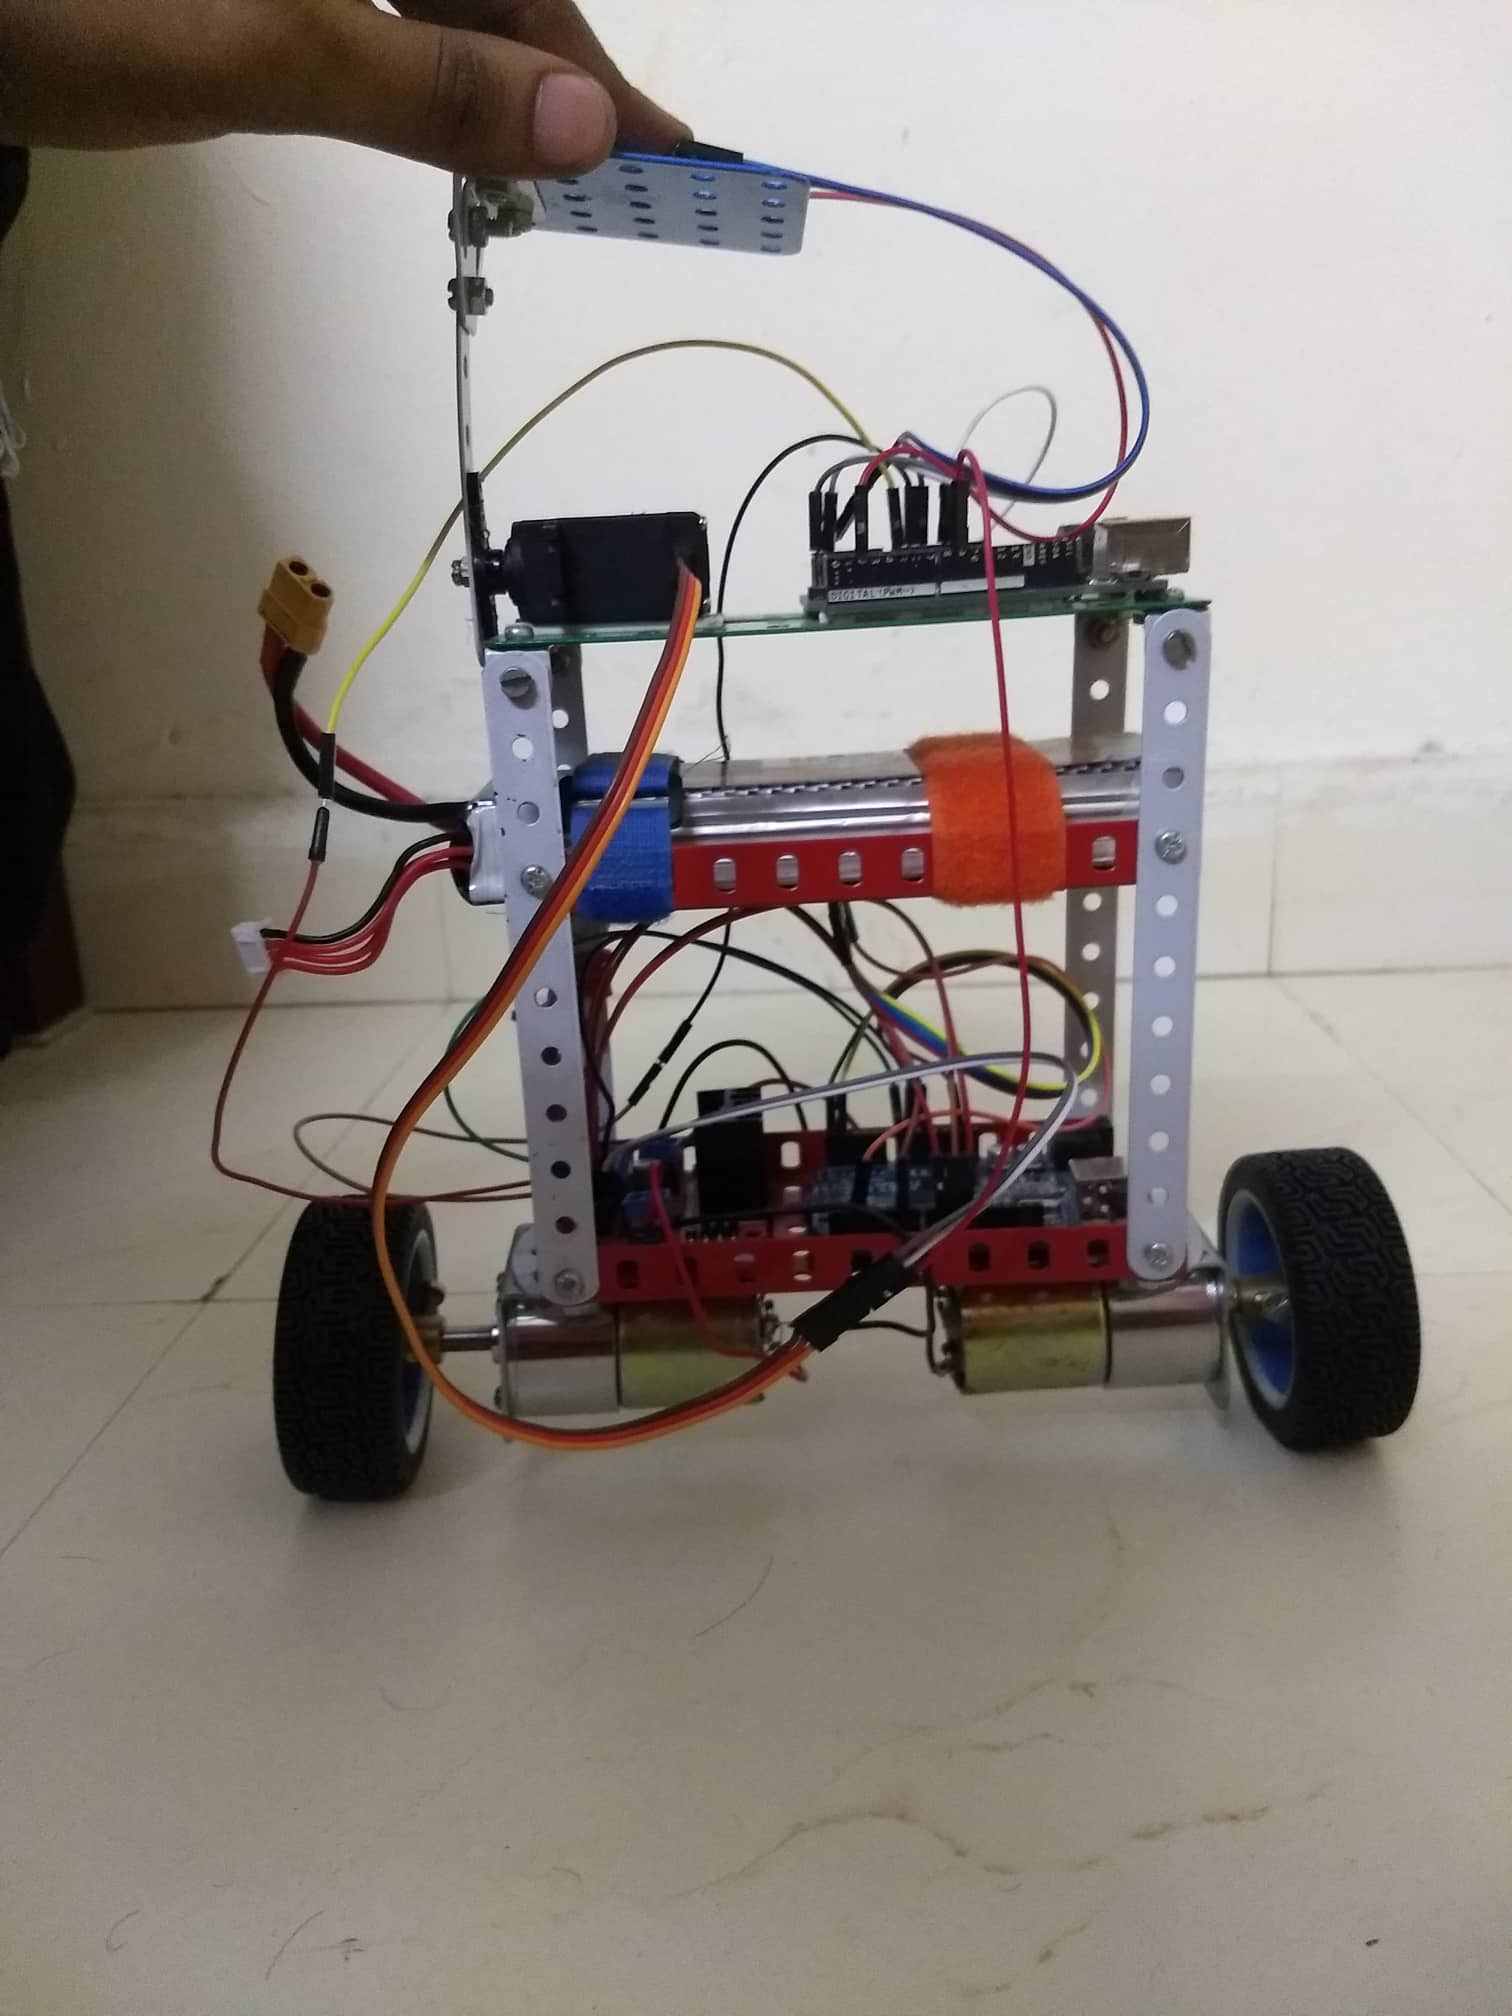
\includegraphics[width=.4\linewidth, scale = 2]{images/bot4}
  \caption{Arrangement of complete bot connections}
  \label{fig:bot2}
\end{subfigure}
\caption{Figure showing the arangement of connections for bot and platform}
\label{fig:combination}
\end{figure}

In figure \ref{fig:combination}, we see the manner in which the prescribed connections are arranged. For the self-balancing table, the arduino is stuck on the top layer of the chassis and the MPU6050 is fixed on top of the platform. \newline
For the self balancing bot, we see from figure \ref{fig:bot2} that the L298N motor driver and the arduino are pasted in the bottom layer of the chassis. The MPU6050 is fixed to the bottom side of the second layer and the battery is placed on the second layer of the chassis.


\chapter{Tuning and operation}
Although the use of the PID algorithm for control does not guarantee optimal control of the system or system stability, it sure is easy to tune.\newline
Steps used in tuning are :
\begin{enumerate}
  \item Set the values of I, D to 0.
  \item Stabilize system as much as possible using only the proportional gain, P.
  \item Set I to remove the steady state error from the system.
  \item Finally, damp the oscillations of the system caused by P by setting D. This helps the bot achieve steady state faster and hence improves response.
\end{enumerate}


\chapter{Future prospects}
After being stabilised by electronics means, self-balancing bots can be loaded with platforms or manipulators, working in human controlled or even completely autonomous operation, and might be used in industrial autonomous transportations systems or warehouses in the future. Models have already been made for employing sleek robots with a low footprint as assistants in hospitals or waiters in restaurants.\\

The use of one variable as the sole manipulator for motion on one axis creates a huge window for simple control by varying the desired setpoint. Better motors (high resolution stepper motors with decent torque) can be implemented to make a smoother and more stable balance system.\\

Different control strategies like State Control or LQR can be experimented with as well as many assumptions can be theorised for better control and stability.


\chapter{Observations and Results}
The bot was stabilized using PID control algorithm. After many trial and error attempts the PID values for which the bot achieved desirable stability are:
\begin{itemize}
  \item P =
  \item I =
  \item D =\\
\end{itemize}

Another important observation from building the bot was that the bot stabilizes faster and in a more desirable manner when the battery is placed not at the bottom but closer to the top of the chassis.


% \bibliographystyle{IEEEtran}
% \bibliography{bibliography/bibliography.bib}
\chapter{Referrences}
[1] F. Grasser, A. D'Arrigo, S. Colombi and A. Rufer, "JOE: a mobile, inverted pendulum", IEEE Transactions on Industrial Electronics, vol. 49, no. 1, pp. 107-114, 2002.\\


\noindent
[2] Peng, K., Ruan, X. and Zuo, G. (2012). Dynamic model and balancing control for two-wheeled self-balancing mobile robot on the slopes. Proceedings of the 10th World Congress on Intelligent Control and Automation.\\
\noindent
[3] B. Mahler, J. Haase, "Mathematical model and control strategy of a two-wheeled self-balancing robot", 39th Annual Conference of the IEEE Industrial Electronics Society IECON 2013, pp. 4198-4203, 2013


%\pagebreak
%\input{chapters/declaration}

\end{document}
